\documentclass[12pt]{article}
\topmargin      =  -15mm
\headheight     =   5mm
\headsep        =   5mm
\oddsidemargin  =    0mm
\evensidemargin =  -10mm
\textwidth      =  160mm
\textheight     =  240mm
\parindent      =    0mm
\parskip        =    3mm

\usepackage{graphicx}
\usepackage{latexsym}
\usepackage{moreverb}
\usepackage{amsmath}
\usepackage{subfigure}
\usepackage{multirow}
\usepackage{hyperref}
\usepackage{shortvrb}
\MakeShortVerb"
\usepackage{xcolor}


\begin{document}

\vspace*{1 cm}
\vskip5cm

\begin{center}

\rule{\textwidth}{1pt}
\LARGE{Chemistry integration with CVODE in PelePhysics} \\ \Large{short note and start guide} \\
\vskip5mm
\Large{Anne Felden  }

\rule{\textwidth}{1pt}\\

\vskip10mm

\large{\textit{\today}}
\end{center}

\newpage
\tableofcontents
\newpage
%==============================
\section{Quickstart}
%==============================
{\color{red} Greetings impatient user. If all you need is a list of keywords and environment variables to perform a simulation with one of the codes available in the \textit{PeleSuite}, then I invite you to directly skip to section~\ref{subs::PPOptions}. If you are in a hurry but still would like more context, visit section~\ref{subs::WD} to be referred to portions of this document that are of interest to you.}


%==============================
\section{Introduction}
%==============================


%=================================
\subsection{Objectives and State-Of-the-Art}
%================================

What we will call the \textit{PeleSuite} (see Fig.~\ref{Fig:PeleSuite}) is currently composed of 3 separate codes:
\begin{itemize}
\item PelePhysics: (\href{https://github.com/AMReX-Combustion/PelePhysics}{see here}) is a repository of physics databases and implementation code for use within the other Pele codes. In particular, the choice of chemistry and transport models as well as associated functions and capabilities are managed in PelePhysics. Follow the link to learn more.
\item PeleLM: (\href{https://github.com/AMReX-Combustion/PeleLM}{see here}) is an adaptive-mesh Low-Mach number hydrodynamics code for reacting flows. Note that by the time this short note is written, PeleLM does \textit{not} rely on PelePhysics yet, and uses in place a \textit{ChemDriver} object. Follow the link to learn more.
\item PeleC: (\href{https://github.com/AMReX-Combustion/PeleC}{see here}) PeleC is an adaptive-mesh compressible hydrodynamics code for reacting flows.
\end{itemize} 
All three codes rely on \href{https://amrex-codes.github.io/amrex/}{AMREX}, which is a software frameworks that provides the data structure and enable massive parallelization.

\begin{figure*}[http]
\centering
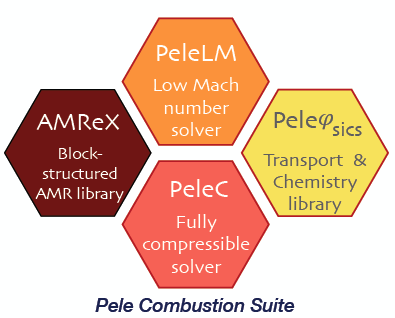
\includegraphics[width=0.4\textwidth]{PeleSuite.png}
\label{Fig:PeleSuite}
\end{figure*}



Up until recently, PelePhysics (as well as the ChemDriver object) depended on DVODE~\cite{VODE:1989} to perform the chemistry integration, no matter the problem at hand. DVODE is a very robust, but slightly outdated, variable-coefficient Ordinary Differential Equation (ODE) solver written in Fortran 77. At its core, it uses a direct dense linear solver. DVODE is very efficient in the resolution of small stiff systems of equations but can become prohibitively expensive when dealing with bigger systems of equations, such as those frequently encountered in combustion systems. In recent years, the Sundials team at LLNL~\cite{hindmarsh2005sundials,cohen1996cvode} have been involved in the active development of a modern, C++ version of DVODE called CVODE. CVODE implements the same functionalities as those available in DVODE, but offers much more flexibility through its user-friendly set of interface routines. Additionally, other linear solvers are available, such as iterative or sparse solvers which can prove to be very efficient in handling "larger" systems of equations~\cite{perini2014study}.

The primary objective of this short note is to explain in details the switch that has been put in motion in the \textit{development} branch of PelePhysics from a DVODE to a CVODE based ODE integration; in terms of:
\begin{itemize}
\item ODE equations solved (\textit{reactor type})
\item Default solver settings chosen (tolerances/order/...)
\item Linear solvers available, along with exemples of performance
\item Changes in PelePhysics run settings
\item Induced changes in the relying codes (such as PeleC)
\end{itemize} 

%===========================
\subsection{What's new chemistry-wise (in a nutshell)}
\label{subs::WD}
%===========================

\textit{Here is a short summary of the functionalities implemented in the PeleSuite of codes. References to sections within the rest of this manuscript are provided, for more insights.}

-- In PelePhysics, \textbf{two different reactor types} have been implemented. The first type is a \textit{constant volume} reactor, were the choice of fixed variables are the internal energy and the density, to comply with PeleC transported variables. This reproduces what was originally implemented with DVODE in PelePhysics. A second reactor type formulated in terms of enthalpy and density has been put in place, to comply with PeleLM. Both reactors are available either via DVODE (in fortran 90) or CVODE (in cpp). See sections~\ref{subs::DiffReacts} for additional details, and~\ref{subs::PPOptions} to see how to activate one or the other via the input files.

-- With both reactors, it is possible to use an \textbf{Analytical Jacobian} (depending upon the choice of linear solver, see section~\ref{sub::LinAlg}.)

-- Three different \textbf{linear solves} can be performed, see section~\ref{sub::LinAlg} for additional details, and~\ref{subs::PPOptions} to see how to make a selection:
\begin{itemize}
\item a dense direct solve
\item a sparse direct solve (requires the KLU library)
\item a sparse iterative solve
\end{itemize} 

-- \textbf{Regression testings} have been put in place in PelePhysics to test the CVODE integration. See section~\ref{subsub::ValidCVreact} for validations, and section~\ref{subs::ReactEvalCvode} for a step-by-step example.

-- A Cvode version running on \textbf{GPU} is currently WIP

-- Many modifications to the chemistry-related routines generator \textbf{Fuego} have been put in place. The one having the largest impact is that the chemistry files are now divided in two parts: a header file "chemistry_file.H" and a C++ file containing the routines definitions. This header file should be imported in any C++ file referencing any Fuego routine. Additionally, a fortran module "fuego_chemistry" is defined that should be imported to use Fuego routines from Fortran.

%=========================================
\section{Introduction to CVODE}
%=========================================
Cvode is part of a software family called sundials for SUite of Nonlinear and DIfferential/ALgebraic equation Solvers~\cite{hindmarsh2005sundials}. Currently, Cvode development version is v5.0.0, while the stable release version is v4.1.0. The version used with PelePhysics is v4.0.2. Cvode can be downladed off of \href{https://computation.llnl.gov/projects/sundials/sundials-software}{the internet}. In the following, details pertaining to the methods implemented in PelePhysics are provided. The interested user is referred to the very exhaustive Cvode User-guide~\cite{CVODE:2019} for more information.

\textit{Most of this section is adapted from the v4.1.0 Cvode Documentation.}

%**************************
\subsection{Numerical method overview}
%**************************

The methods used in Cvode are variable-order, variable-step multistep methods, based on formulas of the form:
\begin{equation}
\sum_{i=0}^{K_1} \alpha_{n,i} y^{n-i} + h_n \sum_{i=0}^{K_2} \beta_{n,i} \dot{y}^{n-i} = 0 
\end{equation}
Here the $y^n$ are computed approximations to $y(t_n)$, and $h_n = t_n-t_{n-1}$ is the step size. For stiff problems, Cvode includes the Backward Differentiation Formulas (BDF) in so-called fixed-leading coefficient (FLC) form, given by $K_1=q$ and $K_2= 0$, with order $q$ varying between 1 and 5.  The coefficients are uniquely determined by the method type, its order, the recent history of the step sizes, and the normalization $\alpha_{n,0}=-1$~\cite{byrne1975polyalgorithm,jackson1980alternative}.  

A nonlinear system must be solved (approximately) at each integration step.  This nonlinear system can be formulated as a  root-finding problem
\begin{equation}
F(y^{n}) = y^n - h_n \beta_{n,0} f(t_n,y^{n}) - a_n = 0
\end{equation}
where $a_n = \sum_{i>0} (\alpha_{n,i} y^{n-i} + h_n\beta_{n,i} \dot{y}^{n-i})$. Cvode provides several non-linear solver choices. By default, Cvode solves this problem with a Newton iteration, which requires the solution of linear systems
\begin{equation}
\label{eq::1}
M[y^{n(m+1)} - y^{n(m)}] = -F(y^{n(m)}) 
\end{equation}
in which
\begin{equation}
M \approx I-\gamma J, \; \; \; J = \frac{\partial f}{ \partial y}, \;\;\; and \;\;\; \gamma =  h_n \beta_{n,0}
\end{equation}


%**************************
\subsection{Linear Algebra}
\label{sub::LinAlg}
%**************************
To find the solution of the linear system~\ref{eq::1}; Cvode provides several linear solver choice. The linear solver modules distributed with Sundials are organized in two families, a \textit{direct} family comprising direct linear solvers for dense, banded, or sparse matrices, and a \textit{spils} family comprising scaled preconditioned iterative (Krylov) linear solvers.  The methods offered through these modules that are of interest in the present document are:
\begin{itemize}
\item dense direct solver
\item sparse direct solver interfaces, in particular using the KLU sparse solver library
\item SPGMR, a scaled -possibly preconditioned- GMRES (Generalized Minimal Residual method) solver~\cite{brown1990hybrid}
\end{itemize}
When using a dense direct solver, the user has the option to specify an analytical Jacobian. If none is provided, a difference quotients is performed. When a sparse direct solver is employed however, the user must specify an analytical Jacobian. All of these options have been enabled in PelePhysics.

For large stiff systems,  where direct methods are often not feasible, the combination of a BDF integrator and a \textit{preconditioned} Krylov method yields a powerful tool. In this case, the linear solve is \textit{matrix-free}, and the default Newton iteration is an Inexact Newton iteration, in which $M$ is applied with matrix-vector products $Jv$ obtained by either difference quotients or a user-supplied routine. In PelePhysics, it is possible to use either a non-preconditioned or a preconditioned GMRES solver. In the latter case, the preconditioner can be either specified in a dense or sparse format (if the KLU library is linked to Cvode), and it is provided in the form of a Jacobian approximation, based on the work of McNenly et al.~\cite{mcnenly2015faster}.

%**************************
\subsection{Error control, step-sizing, order determination}
%**************************

In the process of controlling errors at various levels, Cvode uses  a  weighted  root-mean-square norm, denoted $|| \bullet ||_{WRMS}$, for all error-like quantities. The multiplicative weights used are based on the current solution and on the relative and absolute tolerances input by the user, namely
\begin{equation}
W_i= \frac{1}{[rtol |y_i|+atol_i]}
\end{equation}
Because $1/W_i$ represents a tolerance in the component $y_i$, a vector whose norm is 1 is regarded as small. In PelePhysics, both these tolerances are fixed to a value of 1.0e$-10$.

A critical part of Cvode - making it an ODE \textit{solver} rather than just an ODE method, is its control  of  local  error. At  every  step,  the  local  error  is  estimated  and  required to satisfy tolerance conditions, and the step is redone with reduced step size whenever that error test fails. Note that in PelePhysics, the first time step is always forced to 1.0e$-9$.

In addition to adjusting the step size to meet the local error test, Cvode periodically adjusts the order, with the goal of maximizing the step size. The integration starts out at order 1 and varies the order dynamically after that. The basic idea is to pick the order $q$ for which a polynomial of order $q$ best fits the discrete data involved in the multistep method. In PelePhysics, the maximum order is limited to 2 for stability reasons.

The various algorithmic features of Cvode are inherited from VODE and VODPK, and are documented in~\cite{VODE:1989,brown1990hybrid}.  They are also summarized in the Cvode User-guide~\cite{CVODE:2019} as well as in~\cite{hindmarsh2005sundials}.



%=========================================
\section{Cvode implementation in PelePhysics}
%=========================================

%**************************
\subsection{The different reactors}
\label{subs::DiffReacts}
%**************************
Throughout this document, what we call a \textit{reactor} is in fact a zero-dimensional model, representing the simplest form of a chemically reacting system. Depending upon the choice of state variables driving the system, several different types of reactor can be considered; and the "correct" choice is case dependent. In general, the state variables for a reactor model are
\begin{itemize}
\item The reactor mass
\item The reactor volume
\item The energy of the system
\item The mass fractions for each species
\end{itemize}
The most common type of reactor is the \textit{constant-volume} (CV) reactor, which is the one used to advance the chemistry within PeleC. This reactor type is equivalent to a rigid vessel with fixed volume but variable pressure. In PelePhysics, the constant-volume constraint is ensured by keeping the density $\rho$ fixed -since there is no change of mass; and the indirect choice of energy in the CV reactor implementation is the total energy $E$. $E$'s evolution in our case is solely due to a constant external source term $\dot{E}_{ext}$, which accounts for the effects of advection and convection in the Spectral Deferred Correction (SDC) scheme that all Pele codes use. In that sense, the CV reactor is an abstraction and is not a true closed vessel.

Note that Cvode still integrates the mass fractions ($\rho Y$) together with energy for stability reasons, but a change of variable is applied to effectively transport the temperature $T$ via
\begin{equation}
\rho C_v \frac{\partial T}{\partial t} = \rho\dot{E}_{ext}  - \sum_k e_k {\dot{\omega}_k}^M
\end{equation}
where the $e_k$ are the species internal energy and ${\dot{\omega}_k}^M$ is the species $k$ mass production rate. 

In a second implementation, that we will label \textit{constant-volume-enthalpy} (CVH), the mass-weighted total enthalpy $\rho H$ is used and conserved along with $\rho$. This reactor type is also an abstraction. Here also, $\rho H$ evolves according to an external source term $\dot{\rho H}_{ext}$, and in Cvode, the mass fractions ($\rho Y$) and temperature $T$ are evolved according to
\begin{equation}
\rho C_p \frac{\partial T}{\partial t} = \rho\dot{H}_{ext}  - \sum_k h_k  {\dot{\omega}_k}^M
\end{equation}
where the $h_k$ are the species internal energy. 

%**************************
\subsubsection{Validation of the CV reactor implementation (with CANTERA)}
\label{subsub::ValidCVreact}
%**************************

CANTERA~\cite{cantera} is an open-source suite of tools for problems involving chemical kinetics, thermodynamics, and transport processes. It is a very robust and fast tool written in C++ that is also based on Cvode to perform the chemistry integration. Cvode is well recognized in the combustion community, and by comparing our results to Cantera reactor simulations, we will be able to validate our implementation. 

Note that only the CV reactor model described below can be validated, since as we discussed before, the CVH reactor model is an abstraction needed for our Low-Mach PeleLM chemistry integration. Also, to have a real CV reactor, the external source terms on the energy and species in PelePhysics have been set to 0 (see~\ref{subs::DiffReacts}).

The parameters chosen to initialize the simulation in both Cantera and PelePhysics are described in Table~\ref{table:parameters}. Two sets of runs are performed, with two mechanisms available in PelePhysics. Note that small sub-steps are taken until the final time is reached, but Cvode's internal machinery can subdivides the $dt$ even further. For the purpose of validation, the direct dense solver of Cvode is selected in PelePhysics (see section~\ref{subs::PPOptions}).
\begin{table}
\centering
\begin{tabular}{l c c c c c c}
\hline 
Mechanism          & Mixture                 & T$_0$   & $\phi_0$ & P$_0$          & $dt$              & Final time \\
\hline \hline
Li Dryer               & {$H_2$/$O_2$}    & 1500 K  & 0.8         & 101325 Pa   & 1.0e$-8$ s    & 1.0e$-5$s \\
DRM(TODO)                   & {$CH_4$/$O_2$}  & 1500 K  & 0.8         &  101325 Pa  & ? s &  ? s \\
\end{tabular}
\caption{Initial parameters for the CV reactor simulations.}
\label{table:parameters}
\end{table}

Results are plotted in Fig.~\ref{Fig:MainH2}\&~\ref{Fig:SpecsH2} for the $H_2/O_2$ mixture. All curves are indistinguishable, so the relative error of all major quantities is also plotted in Fig.~\ref{Fig:ErrH2}. Note that $H_2$ and $O_2$ relative errors have similar features, and that relative errors observed for $H$ and $H_2O$ are representative of those exhibited by, respectively, intermediates and products.

\begin{figure*}[http]
\centering
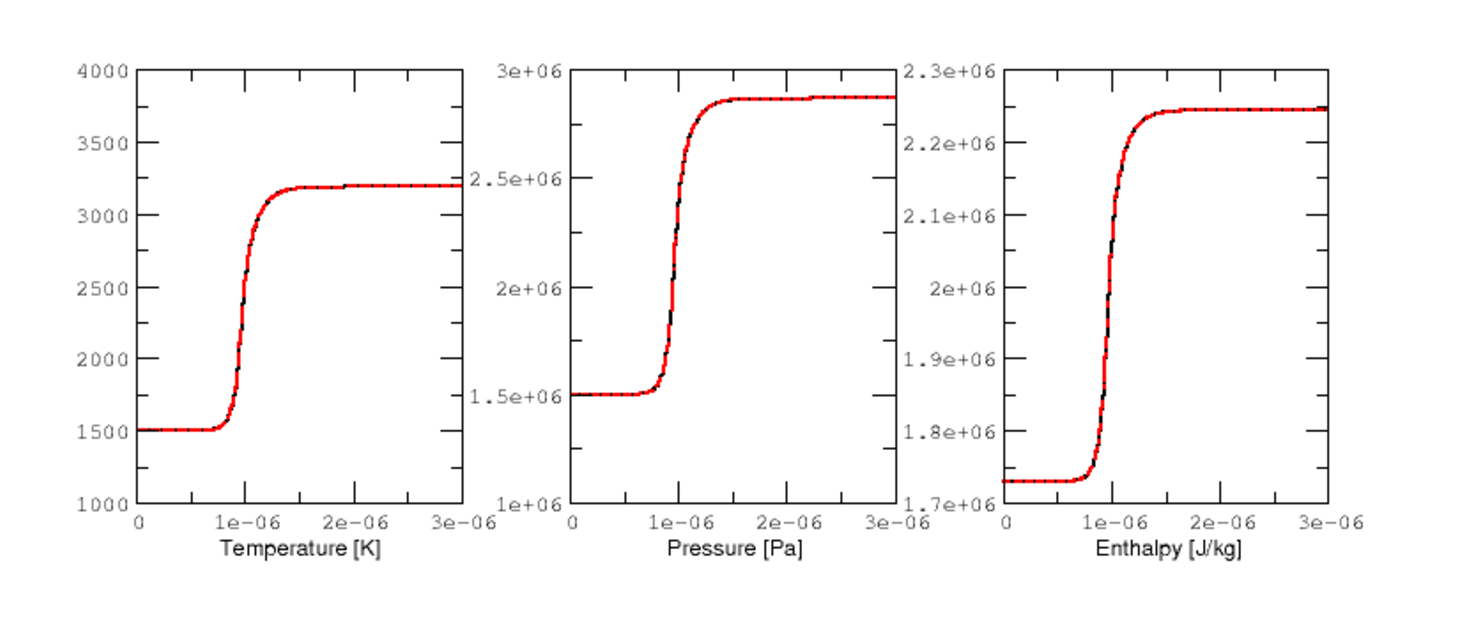
\includegraphics[width=1.\textwidth]{Main_pdf.pdf}
\caption{Evolution of temperature, pressure and enthalpy in a CV reactor, computed with the LiDryer mechanism. Black: CANTERA, red: PelePhysics.}
\label{Fig:MainH2}
\end{figure*}

\begin{figure*}
\centering
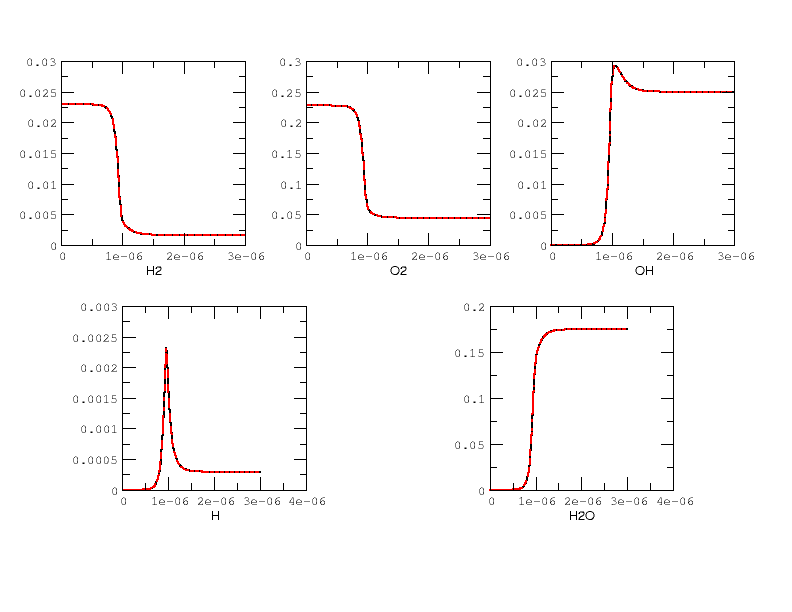
\includegraphics[width=1.\textwidth]{Specs.png}
\caption{Evolution of major species in a CV reactor, computed with the LiDryer mechanism. Black: CANTERA, red: PelePhysics.}
\label{Fig:SpecsH2}
\end{figure*}

\begin{figure*}
\centering
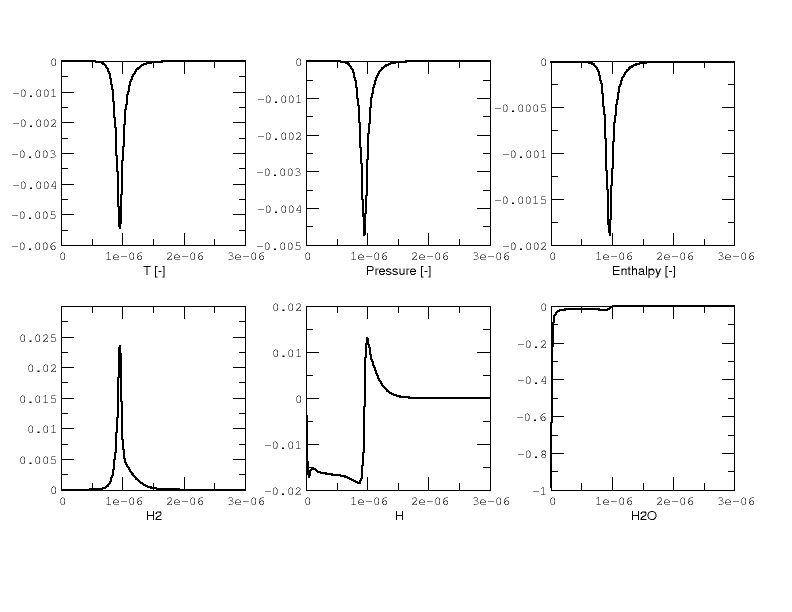
\includegraphics[width=1.\textwidth]{ERRs.png}
\caption{Relative errors on the temperature, pressure, enthalpy and major species in a CV reactor, computed with the LiDryer mechanism.}
\label{Fig:ErrH2}
\end{figure*}

Overall, considering the many Cvode controlling parameters, results are deemed acceptable and that concludes the validation of the reactors implementations in PelePhysics.

%**************************
\subsection{Activating the different options via the input files}
\label{subs::PPOptions}
%**************************
Choosing between DVODE/Cvode is done at compile time, via the GNUmakefile. On the other hand, the type of reactor and numerical algorithm are selected via keywords in the input file. There is a subtlety though: when any sparsity feature is required, the choice should also be made a compile time; and if the option is not selected, subsequent options via keywords can either lead to an error or fall back to a dense formulation of the problem. This is discussed in more depth in what follows.

%****
\subsubsection{Preliminary step: Cvode and SuiteSparse}
%****
\textbf{The user is in charge of installing the proper Cvode version, as well as installing and properly linking the KLU library if sparsity features are needed.}

As previously said, the \textbf{Cvode version} employed to perform all tests presented in this document is \textbf{v4.0.2}. Cvode can be downloaded by following \href{https://computation.llnl.gov/projects/sundials/sundials-software}{this link}. \\ 
An "INSTALL_GUIDE.pdf" will be present in the source files, explaining how to properly install and build the needed librairies. If the KLU library is to be used, then the proper flags should be set. With the version sub-mentioned, those are "-DKLU_ENABLE" (should be set to "ON")  "-DKLU_INCLUDE_DIR" (should point to the location where your "klu.h" file is) and "-DKLU_LIBRARY_DIR" (which should point to the location where your KLU library was generated). 

The \textbf{KLU library is part of the \textit{SuiteSparse} distribution}~\cite{SuiteSparse:2019} that can be downloaded~\href{http://faculty.cse.tamu.edu/davis/suitesparse.html}{following this link}. The SuiteSparse version used for all tests presented in this document is \textbf{v4.5.0}, and we do not guarantee that the linking will properly work with subsequent releases. A "README" file will explain how to generate the KLU library.

Once Cvode has been build and installed -with proper linking to the KLU library if necessary, \textbf{the CVODE\_LIB\_DIR environment variable should be set, pointing towards the location where all Cvode libraries have been generated}.

%****
\subsubsection{The GNUmakefile}
\label{subsubs::GNUtype}
%****
The default setting is to use DVODE in PelePhysics; i.e, if no modifications are done to the original GNUmakefile, then this option should automatically be selected. To activate Cvode, the following line should be added:
\begin{verbatim}
USE_SUNDIALS_3x4x = TRUE
\end{verbatim}
Note that this is an AMREX flag, so it will automatically be recognized throughout the Pele codes. 

If sparsity features are required, then the following line should also be added:
\begin{verbatim}
USE_KLU = TRUE
ifeq ($(USE_KLU), TRUE)  
        DEFINES  += -DUSE_KLU
endif
\end{verbatim}
In this case, the location of the "klu.h" should be specified via:
\begin{verbatim}
INCLUDE_LOCATIONS += path_to_your_klu.h
\end{verbatim}
The only place where this flag will be used is in the C++ file where all Cvode calls are done.

%****
\subsubsection{The input file}
%****
If DVODE is chosen, no modifications of the input file are required. If Cvode is selected, then the original input file will trigger a dense direct solve without Analytical Jacobian. Three keywords control the algorithm.
\begin{itemize}
\item "cvode_iE" enable to switch from a CV reactor ("1") to a CVH reactor ("2").
\item "ns.cvode_iDense" controls the numerical method: choose "1" to enable the dense direct linear solver, "5" for the sparse direct linear solver (if the KLU library has been linked) and "99" for the Krylov iterative solver
\item "ns.cvode_iJac" is a bit less obvious. If "ns.cvode_iDense = 1", then "ns.cvode_iJac = 1" will activate the use of an Analytical Jacobian. But if "ns.cvode_iDense = 99", then "ns.cvode_iJac = 1" will activate the preconditioned GMRES solver while "ns.cvode_iJac = 0" will activate the non-preconditioned GMRES solver. Additionally, if "ns.cvode_iDense = 99", "ns.cvode_iJac = 1" and the KLU library is linked, then the preconditioned solve is done in a sparse format. Note that with "ns.cvode_iDense = 5", the only allowed option is "ns.cvode_iJac = 1".
\end{itemize}


%**************************
\subsection{The ReactEvalCVODE test case in details}
\label{subs::ReactEvalCvode}
%**************************
This tutorial has been adapted from the ReactEval tutorial employed in the series of regression tests to monitor the DVODE chemistry integration. The domain considered is a 2x1024x2 box, where the initial temperature is different in each $(i,j,k)-$ cell, according to a $y-$ evolving sinusoidal profile (see Fig.~\ref{Fig:ErrH2}):
\begin{equation}
T(i,j,k) =  T_l + (T_h-T_l)\frac{y(i,j,k)}{L} + dTsin\left(2\pi\frac{y(i,j,k)}{P}\right) 
\end{equation}
The different parameters involved are summarized in Table~\ref{Tab::ParamReactEvalCvode}. The initial composition is the same in every cell, and is a mixture of 0.1  $CH_4$, 0.2 $O_2$ and 0.7 $N_2$ in mass fractions. The initial pressure is 1 atm and the mechanism considered is the DRM mechanism.

\begin{table}
\centering
\begin{tabular}{c c c c c}
\hline 
$T_l$                 & $T_h$            & $dT$              & $L$    & $P$           \\
\hline \hline
2000 K               & 2500 K           & 100 K            & 1024         &  $L/4$ \\
\end{tabular}
\caption{Parameters used to initialize T in the ReactEvalCVODE test case.}
\label{Tab::ParamReactEvalCvode}
\end{table}

\begin{figure*}
\centering
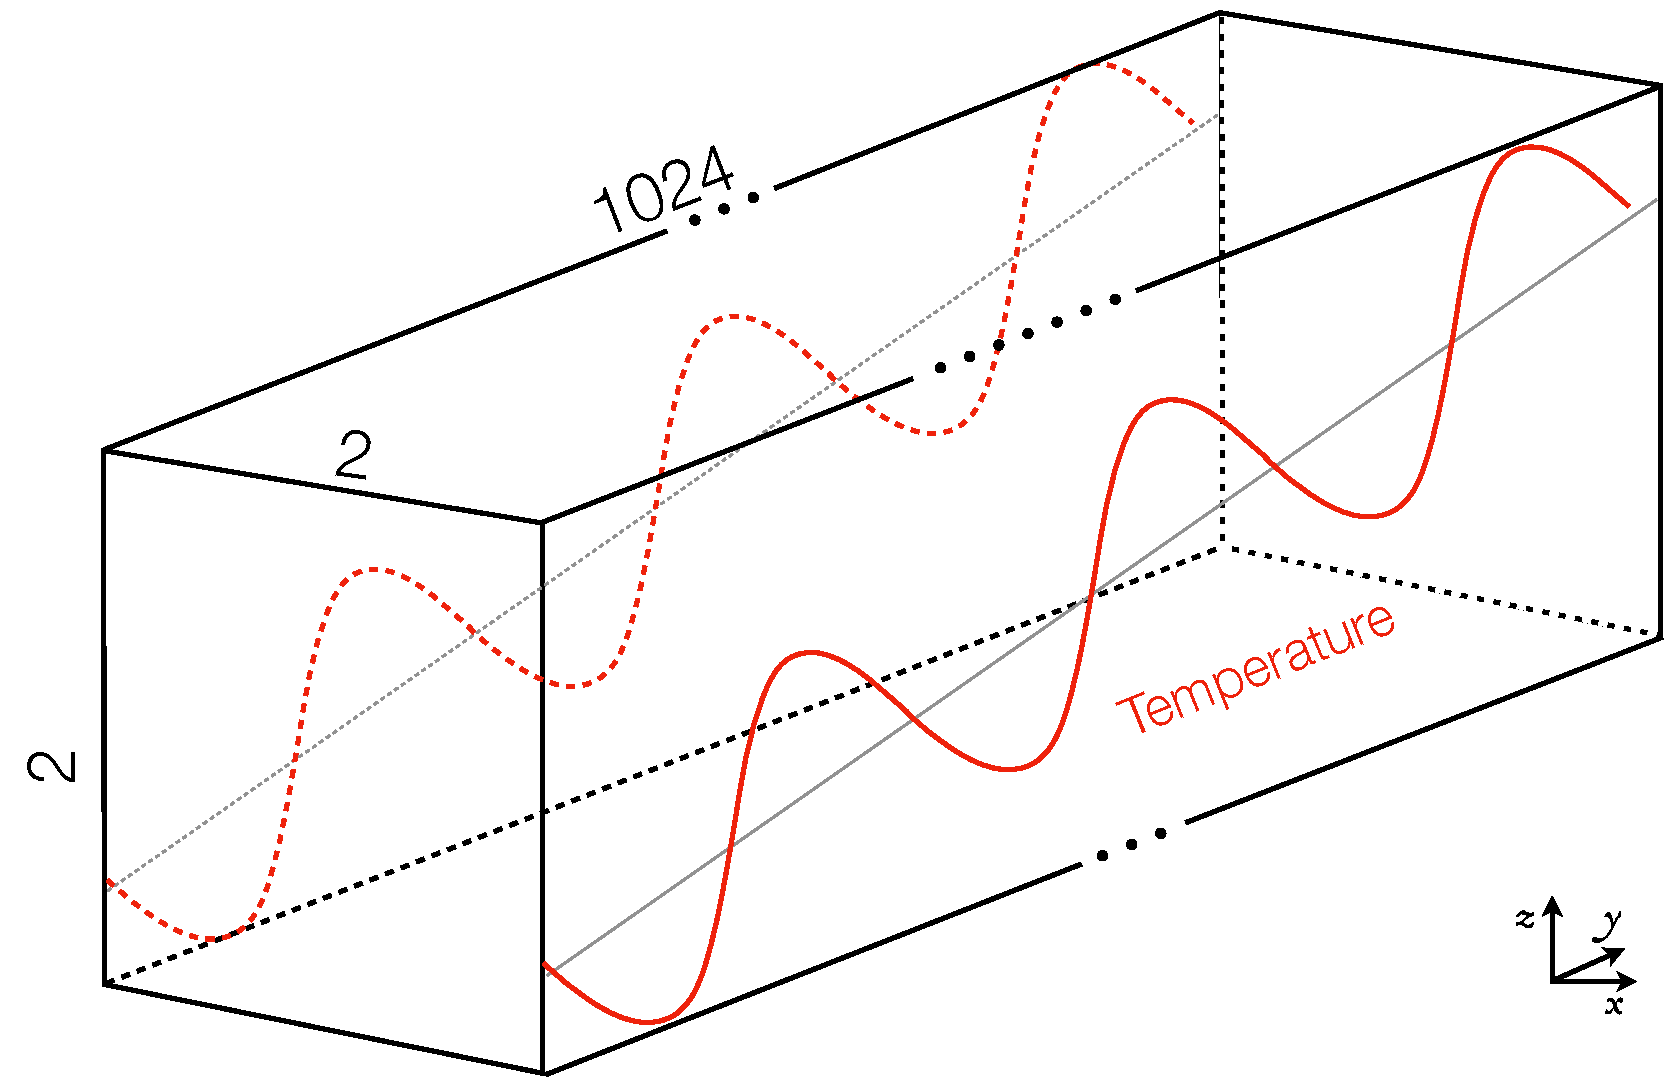
\includegraphics[width=0.5\textwidth]{Case_ReactEvalCvode.pdf}
\caption{The ReactEvalCVODE test case.}
\label{Fig:ErrH2}
\end{figure*}

%****
\subsubsection{The input files}
%****
The run parameters that can be controlled via the input files are as follows
\begin{verbatim}
dt = 1.e-05  
ndt = 100
cvode_ncells = 1

cvode_iE = 1
ns.cvode_iDense = 1
ns.cvode_iJac = 0

amr.plot_file       = plt
\end{verbatim}
so in this example, a CV reactor model is chosen to integrate each cell, and the dense direct solve without analytical Jacobian is activated. Each cell is then integrated for a total of 1.$e-05$ seconds, with 100 external time steps. This means that the actual $dt$ is 1.$e-07$, a little more than what is used in the PeleC code, but consistent with what will be used in PeleLM. The number of cells to be integrated simultaneously is 1~\footnote{NOTE that only one cell at a time should be integrated with Cvode right now. The vectorized version on CPU is still WIP and not properly implemented for all linear solver}.

%****
\subsubsection{The GNUmakefile}
%****
For this example, the "USE_SUNDIALS_3x4x" flag should be set to true, as the ODE integration is called from the C++ routine directly and will thus not work with DVODE (only accessible via FORTRAN with the current implementation).

Additionally, the "FUEGO" file should be set to true and the chemistry model should be set to "drm19". The full file reads as follows
\begin{verbatim}
PRECISION  = DOUBLE                                                                                                                   
PROFILE    = FALSE

DEBUG      = TRUE

DIM        = 3

COMP       = gcc
FCOMP      = gfortran

USE_MPI    = TRUE
USE_OMP    = FALSE

FUEGO_GAS  = TRUE

# define the location of the PELE_PHYSICS top directory
PELE_PHYSICS_HOME    := ../../../..

#######################
USE_SUNDIALS_3x4x = TRUE

USE_KLU = FALSE
ifeq ($(USE_KLU), TRUE)
    DEFINES  += -DUSE_KLU
    include Make.CVODE
endif

#######################
ifeq ($(FUEGO_GAS), TRUE)
  Eos_Model       = Fuego
  Chemistry_Model = drm19
  Reactions_dir   = Fuego
  Transport_Model = Simple
else
  Eos_Model       = GammaLaw
  Reactions_dir   = Null
  Transport_Model = Constant
endif

Bpack   := ./Make.package
Blocs   := .

include $(PELE_PHYSICS_HOME)/Testing/Exec/Make.PelePhysics         
\end{verbatim}
where the "Make.CVODE" contains the link to the SuiteSparse include files (see Section~\ref{subsubs::GNUtype})

%****
\subsubsection{Results}
%****
It took 2m44s to integrate the 4096 cells of this box, with 4 MPI processes and no OMP process. The resulting temperature evolution for all cells is displayed in Fig~\ref{Fig:ReacEvalCv}.

\begin{figure*}[http]
\centering
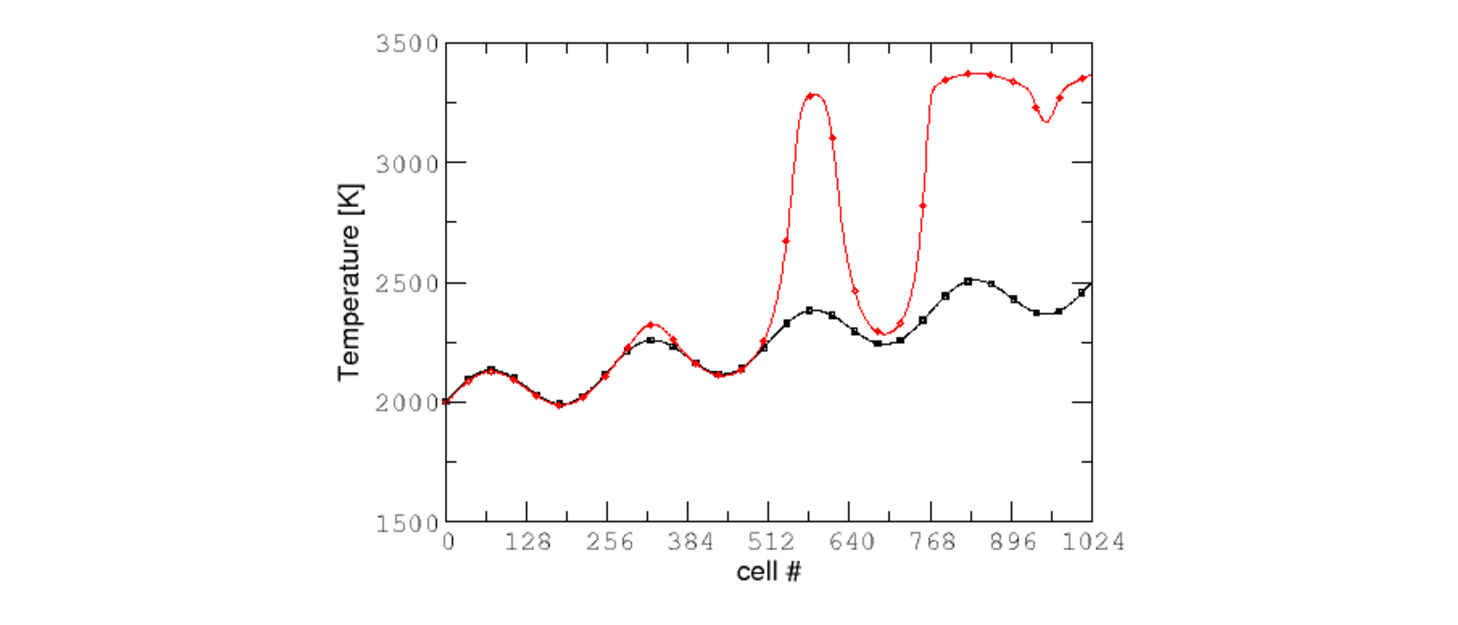
\includegraphics[width=1.\textwidth]{ReactEvalCv.pdf}
\caption{Evolution of temperature in the 2x1024x2 example box, using a CV reactor and a dense direct solve, and computed with the DRM mechanism. Black: $t=0$, red: $t=1e-05s$.}
\label{Fig:ReacEvalCv}
\end{figure*}

%**************************
\subsection{To go further: ReactEvalCVODE with the KLU library}
\label{subs::ReactEvalCVODEKLU}
%**************************
%****
\subsubsection{The input files}
%****
For the KLU library to be of use, a solver utilizing sparsity features should be selected. We modify the input file as follows
\begin{verbatim}
dt = 1.e-05  
ndt = 100
cvode_ncells = 1

cvode_iE = 1
ns.cvode_iDense = 99
ns.cvode_iJac = 1

amr.plot_file       = plt
\end{verbatim}
So that now, a preconditioned iterative Krylov solver is selected, where the preconditioner is specified in a sparse format.

%****
\subsubsection{The GNUmakefile}
%****
Only the middle part of the GNUmakefile is modified compared to the previous example, section~\ref{subs::ReactEvalCvode}.
\begin{verbatim}
...
#######################
USE_SUNDIALS_3x4x = TRUE

USE_KLU = TRUE
ifeq ($(USE_KLU), TRUE)
    DEFINES  += -DUSE_KLU
    include Make.CVODE
endif

#######################
...
\end{verbatim}

%****
\subsubsection{Results}
%****
This run now takes 3m29s to run. As expected from the dense Jacobian of the system obtained when using the small DRM mechanism (the fill in pattern is $>90 \%$), using an iterative solver does not enable to reach speed-ups over the simple dense direct solve used in section~\ref{subs::ReactEvalCvode}. NOTE, and this is important, that this tendency will revert when sufficiently small time steps are used. For example, if instead of $1e-7s$ we took time steps of $1e-8s$ (consistent with PeleC time steps), then using the iterative GMRES solver would have provided significant time savings. This is because the smaller the time step the closer the system matrix is from the identity matrix and the GMRES iterations become really easy to complete.

This example illustrates that choosing the ''best'' and ''most efficient'' algorithm is far from being a trivial task, and depends upon many factors. Table~\ref{Tab::RunsReactEvalCvode} provides a summary of the run time in solving the ReactEvalCVODE example with the various available Cvode linear solvers.

\begin{table}
\centering
\begin{tabular}{l c c c c c}
\hline 
Solver                   & Direct               & Direct               & Direct                         & Iter.                      &   Iter.      \\
                             & Dense              & Sparse AJ             & Dense AJ                  & Precond. (D)               & Precond. (S)    \\
KLU                      &     OFF              &   ON                  & OFF                               & OFF                   &  ON              \\
\hline 
"cvode_iE"              & 1                      &     1                     & 1                                    & 1                        &  1      \\
"ns.cvode_iDense" & 1                      &    5                      & 1                                    & 99                      &  99 \\ 
"ns.cvode_iJac"      & 0                      &    1                      & 1                                    & 1                        &  1 \\ 
\hline
Run time $[s]$      &  2m44s           & 1m59s                      & 1m42s                           & 3m05s                    &  3m29s   \\
\end{tabular}
\caption{Summary of ReactEvalCvode runs with various algorithms.}
\label{Tab::RunsReactEvalCvode}
\end{table}


%**************************
\subsection{Current Limitations}
%**************************

%**************************
\subsection{Tricks and hacks, stuff to know}
\label{subs::Tricks}
%**************************
When using DVODE, there is a ''hack'' enabling the user to reuse the Jacobian instead of reevaluating it from scratch. This option is triggered when setting the "extern_probin_module" flag "new_Jacobian_each_cell" to 0. This can be done in PelePhysics (in the ReactEval test folder for example) by adding the following line in the "probin" file
\begin{verbatim}
&extern
 new_Jacobian_each_cell = 1                                                                                                           
/
\end{verbatim}

A similar feature is currently not available in Cvode, although it would be possible to modify the "CVodeReInit" function to reinitialize only a subset of counters. This is currently under investigation. The user still has some control via the Cvode flag "CVodeSetMaxStepsBetweenJac".

Note that Cvode is currently \textit{NOT} guaranteed to work with OMP !! It will however work (as seen on the previous examples) with MPI.

%**************************
\subsection{How does Cvode compare with DVODE ?}
%**************************
Depending on whether the famous AJ ''hack'' is activated or not in DVODE, the run can be much faster with DVODE. The same test case as that described in section~\ref{subs::ReactEvalCvode} can also be integrated with DVODE. We will call this test case ReactEvalDVODE. Note that this test case is slightly different from the famous ReactEval. Only the GNUmakefile needs to be modified
\begin{verbatim}
...
#######################
USE_SUNDIALS_3x4x = FALSE

USE_KLU = FALSE
ifeq ($(USE_KLU), TRUE)
    DEFINES  += -DUSE_KLU
    include Make.CVODE
endif

#######################
...
\end{verbatim}
and, as explained in section~\ref{subs::Tricks}, the famous AJ ''hack'' can be activated via the "probin" file.

Two runs are performed, activating the hack or not. Times are reported in Table~\ref{Tab::CVODEvsDVODE}.
\begin{table}
\centering
\begin{tabular}{l c c c}
\hline 
Solver                            & Direct               & Direct               & Direct                                          \\
                                      & Dense              & Dense              & Dense + AJ \textit{hack}              \\
KLU                               &     OFF             &   OFF                  & OFF                                     \\
"USE_SUNDIALS_3x4x" &     ON               &   OFF                  & OFF                                   \\  
\hline 
"cvode_iE"              & 1                      &     1                         & 1                                         \\
"ns.cvode_iDense" & 1                      &    N/A                      & N/A                                     \\
"ns.cvode_iJac"      & 0                      &    N/A                      & N/A                                 \\
\hline
Run time $[s]$      &  2m44s           & 4m49s                     & 4m00s                             \\
\end{tabular}
\caption{Summary of ReactEvalCvode run vs ReactEvalDVODE.}
\label{Tab::CVODEvsDVODE}
\end{table}


%=========================================
\section{PeleC with Cvode via PelePhysics}
%=========================================

%=========================================
\section{Cvode on GPU: the ReactEvalCVODEGPU test case (WIP) }
%=========================================

\clearpage
\input{./journaux.tex}
\bibliographystyle{unsrt}
\bibliography{Biblio.bib}
%\bibliography{./COMB_STD-Sep16}

\end{document}
